\documentclass[tikz]{standalone}
\usetikzlibrary{calc,trees,positioning,arrows,chains,shapes.geometric,%
    decorations.pathreplacing,decorations.pathmorphing,shapes,%
    matrix,shapes.symbols,fit}

\pgfdeclarelayer{back}
\pgfsetlayers{back,main}


\makeatletter
\tikzset{
  fitting node/.style={
    inner sep=0pt,
    fill=none,
    draw=none,
    reset transform,
    fit={(\pgf@pathminx,\pgf@pathminy) (\pgf@pathmaxx,\pgf@pathmaxy)}
  },
  reset transform/.code={\pgftransformreset}
}
\makeatother


\begin{document}
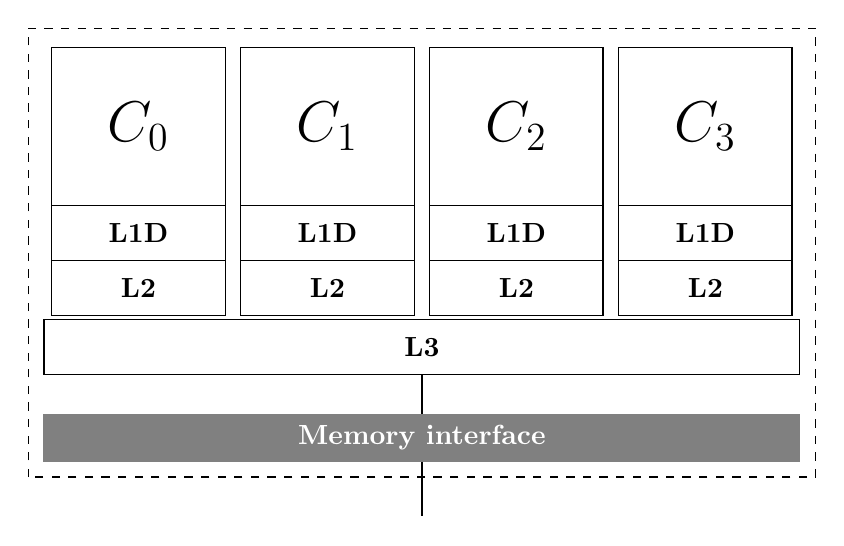
\begin{tikzpicture}
  \draw[dashed] (0,0) rectangle (10,5.7) node[fitting node] (cpu_envelope) {};
  
  \draw[-,fill=gray,draw=gray] (0.2,.2) rectangle (9.8,.8) node[fitting node] (meminterface) {};
  \node (meminterface_label) [text=white] at(meminterface) {\bfseries{}Memory interface};
  \draw[-] (0.2,1.3) rectangle (9.8,2) node[fitting node] (l3) {};
  
  \node (l3_label) [text=black] at(l3) {\bfseries{}L3};
  \path (l3) edge[-,thick] (meminterface.north) %
  (meminterface.south) edge[-,thick] ([yshift=-1cm]meminterface);  
  
  \foreach \c in {0,...,3}
  {
    %\draw[-] ($(0.2,2.05)+(2.4*\c,0)$) rectangle ($(2.3,2.75)+(2.4*\c,0)$) node[fitting node] (l2_\c) {\bfseries{}L2};
    \node [draw,rectangle, minimum width=2.2cm, minimum height=.7cm] at($(1.4,2.4)+(2.4*\c,0)$) {\bfseries{}L2};
    \node [draw,rectangle, minimum width=2.2cm, minimum height=.7cm] at($(1.4,3.1)+(2.4*\c,0)$) {\bfseries{}L1D};
    \node [draw,rectangle, minimum width=2.2cm, minimum height=2cm,font=\huge] at($(1.4,4.45)+(2.4*\c,0)$) {$C_\c$};
  }

  \end{tikzpicture}
\end{document}
